\section{Training Approach}

\begin{outline}
  Describe the reinforcement learning or supervised learning approach
  used to train the CNN models.
\end{outline}

The factors that make up the footstep cost maps in the training data
are shown in \ref{fig:costmap-composition-elements}, while the
combined cost map is shown in \ref{fig:costmap-composition-combined}.
The most significant factors are the support polygon stability,
measured as the distance from the COM to the nearest edge of the
support polygon (\textit{inscribed\_circle\_radius}), and the
distance from the nominal foot position
(\textit{foot\_hip\_distance}). Other factors make up a small, but
still important part of the cost map. These include
\textit{lin\_vel\_z\_l2} which penalizes high vertical velocity,
\textit{ang\_vel\_xy\_l2} which penalizes high angular velocity in
the horizontal plane, \textit{joint\_torques\_l2} which penalizes
high joint torques, \textit{joint\_acc\_l2} which penalizes high
joint accelerations, and \textit{control\_error}, which penalizes
errors in the swing duration between the requested and actual values.
Some of these factors are balanced to have a lower spread, mitigating
factors that consistently prefer one leg over another.

\begin{figure}
  \centering
  \begin{subfigure}[T]{0.65\textwidth}
    \centering
    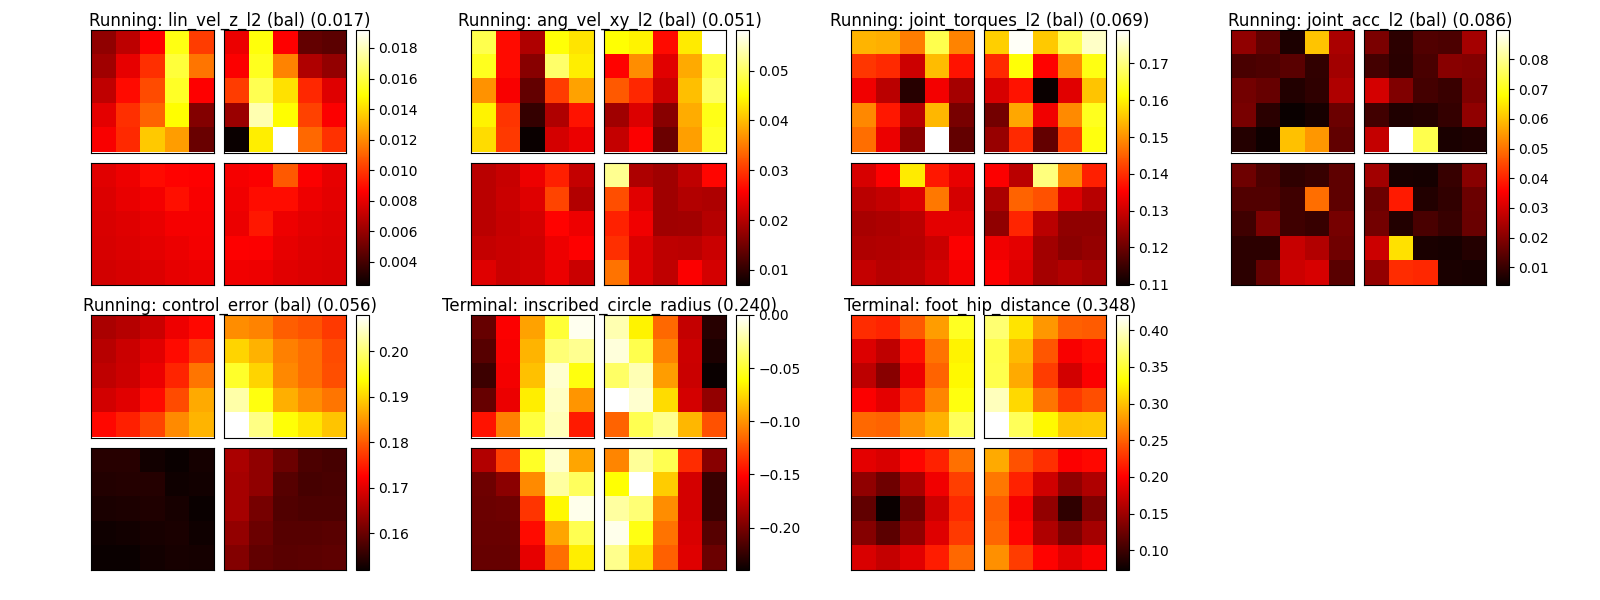
\includegraphics[width=\textwidth]{images/data/training/costmap-composition/elements.png}
    \caption{Factors influencing footstep cost maps. \textit{(bal)}
      indicates that the values for each leg were balanced to have a
      lower spread, mitigating factors that consistently prefer one leg
      over another. The last number in parenthesis indicates the total
    range of the data, the most important factor for the combined cost map.}
    \label{fig:costmap-composition-elements}
  \end{subfigure}
  \hfill
  \begin{subfigure}[T]{0.3\textwidth}
    \centering
    \includegraphics[width=\textwidth]{images/data/training/costmap-composition/combined.png}
    \caption{Combined cost map from factors in (a).}
    \label{fig:costmap-composition-combined}
  \end{subfigure}
  \hfill
\end{figure}

\begin{figure}
  \centering
  \includegraphics[width=0.8\textwidth]{images/data/training/training-fl-sweep.png}
  \caption{Snapshot showing 25 robots testing different footstep
    positions in parallel. For real data generation, 100 are run in
  parallel, testing 25 footstep positions for each foot at a time.}
\end{figure}

\begin{figure}
  \centering
  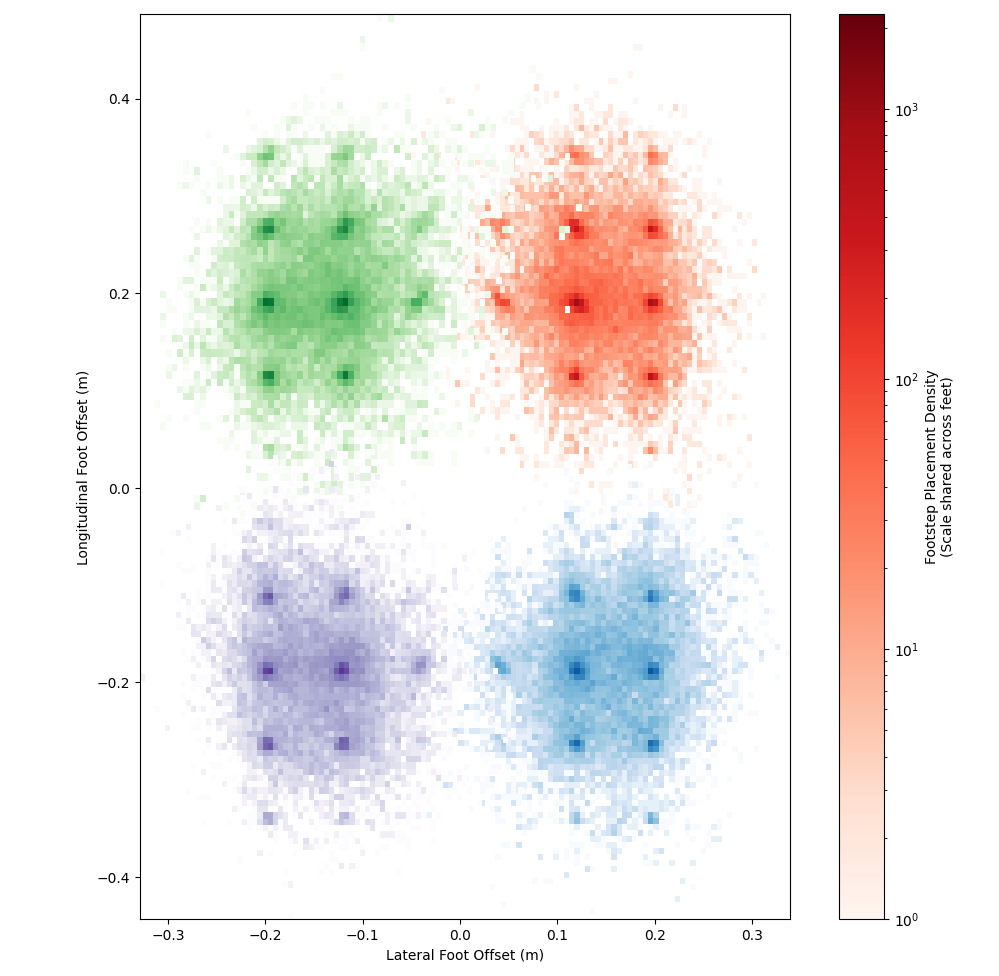
\includegraphics[width=0.8\textwidth]{images/data/foot-placement-heatmaps.png}
  \caption{Foot placement heatmaps showing distribution of foot
    positions in the GaitNet training data. Note that the histograms
  are overlaid in some places, obscuring data underneath.}
  \label{fig:data-cn-training-process}
\end{figure}

As in \cite{bratta_contactnet_2024}, the cost maps are normalized to
improve training performance. Our approach differs in how the cost
maps are normalized though. We directly normalize the cost maps to
the range $[0, 1]$, whereas \cite{bratta_contactnet_2024} normalizes
to $[0,1]$ in such a way that only the relative ordering of costs are
preserved. This difference is critical to our system to provide the
upstream GaitNet model with as much information as possible.

Below is the equation used as the input to the contact model.

\[
  \mathbf{x} =
  \begin{bmatrix}
    \mathbf p_{b,xy} \\
    \mathbf r_{w,z} \\
    \mathbf v_b \\
    \mathbf \omega_b \\
    \mathbf u
  \end{bmatrix}
\]

where
$\mathbf p_{b,xy}$ is the $x$ and $y$ position all end effectors in
the base frame stacked into a single vector,
$\mathbf r_{w,z}$ is the height of the robot's COM in the world frame.

The model is trained on $y$, the heuristically calculated footstep
cost maps (\autoref{fig:data-footstep-cost-map}).

\begin{figure}
  \centering
  \includegraphics[width=0.75\linewidth]{images/data/footstep-cost-map.png}
  \caption{Footstep cost map. Shows the heuristic cost for each
  possible footstep location.}
  \label{fig:data-footstep-cost-map}
\end{figure}

Here, the inclusion of $\mathbf \omega_b$ differs from
\cite{bratta_contactnet_2024}

The results of this model are very promising, with the model able to
predict footstep cost maps with high accuracy.
\autoref{fig:data-cn-typical-comparison}
shows the model output and ground truth for typical data sample.
\autoref{fig:data-cn-challenging-comparison}
shows a particularly challenging data sample, and the model is still
able to identify the best positions for each leg,
particularly the back left leg, which needs to be far from the
nominal position to maintain stability in that state.

\begin{figure}
  \centering
  \begin{minipage}[T]{0.45\textwidth}
    \centering
    \includegraphics[width=\textwidth]{images/data/training/typical-expected.png}
  \end{minipage}
  \hfill
  \begin{minipage}[T]{0.45\textwidth}
    \centering
    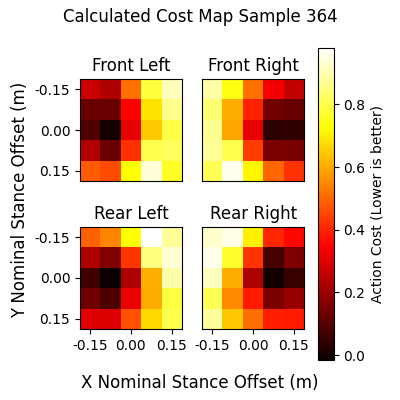
\includegraphics[width=\textwidth]{images/data/training/typical-calculated.png}
  \end{minipage}
  \hfill

  \caption{Typical data samples showing calculated (left) and
  expected (right) quadruped images.}
  \label{fig:data-cn-typical-comparison}
\end{figure}

\begin{figure}
  \centering
  \begin{minipage}[T]{0.45\textwidth}
    \centering
    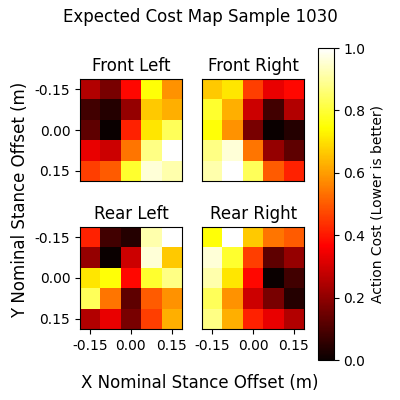
\includegraphics[width=\textwidth]{images/data/training/challenging-expected.png}
  \end{minipage}
  \hfill
  \begin{minipage}[T]{0.45\textwidth}
    \centering
    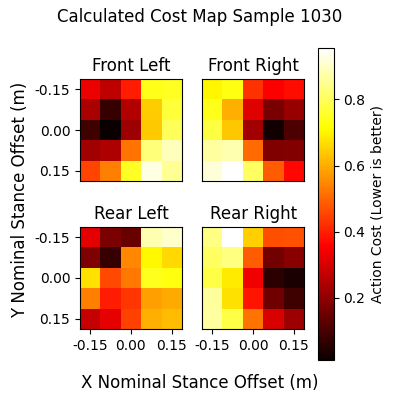
\includegraphics[width=\textwidth]{images/data/training/challenging-calculated.png}
  \end{minipage}
  \hfill

  \caption{Particularly challenging data samples showing calculated (left) and
  expected (right) quadruped images.}
  \label{fig:data-cn-challenging-comparison}
\end{figure}
